%%
%% AEGIS-Dengue full paper. Revised 30 September 2026 after the literature review of
%% 29 September 2026. Every benchmark number is taken from results/benchmark/tables/*.csv
%% and results/benchmark/onset_task/*.csv, built on one frozen climate file
%% (results/benchmark/data_manifest.json); Table 2 (the earlier one-week study) is
%% from the short paper's verified tables. Figures: copy results/benchmark/figures/*.pdf
%% and figures/fig_h1_landscape.pdf into figures/ (or images/ on Overleaf).
%%
% The bibliography is embedded so this single file compiles on its own (Prism,
% Overleaf or a local install): LaTeX writes references_long.bib on the first run.
\begin{filecontents*}[overwrite]{references_long.bib}
%% Bibliography for docs/full paper.tex.
%% The first eight entries are the short paper's references (reconstructed from its
%% printed reference list; replace them with the Overleaf references.bib entries if
%% those differ). The four entries flagged VERIFY in the earlier draft (Liu et al.,
%% the global ensemble study, the Brazil sprint and Chronos-2) were resolved in the
%% literature review of 29 September 2026, which also supplied the new keys below.
%% Fields the review did not state (volume, pages) are left out rather than guessed.

@inproceedings{cho2014gru,
  author    = {Kyunghyun Cho and Bart van Merri{\"e}nboer and Caglar Gulcehre and Dzmitry Bahdanau and Fethi Bougares and Holger Schwenk and Yoshua Bengio},
  title     = {Learning Phrase Representations using {RNN} Encoder--Decoder for Statistical Machine Translation},
  booktitle = {Proceedings of the 2014 Conference on Empirical Methods in Natural Language Processing (EMNLP)},
  pages     = {1724--1734},
  year      = {2014},
  doi       = {10.3115/v1/D14-1179}
}

@article{funk2015chirps,
  author  = {Chris Funk and Pete Peterson and Martin Landsfeld and Diego Pedreros and James Verdin and others},
  title   = {The Climate Hazards Infrared Precipitation with Stations---A New Environmental Record for Monitoring Extremes},
  journal = {Scientific Data},
  volume  = {2},
  pages   = {150066},
  year    = {2015},
  doi     = {10.1038/sdata.2015.66}
}

@inproceedings{kingma2015adam,
  author    = {Diederik P. Kingma and Jimmy Ba},
  title     = {Adam: A Method for Stochastic Optimization},
  booktitle = {International Conference on Learning Representations (ICLR)},
  year      = {2015}
}

@inproceedings{kipf2017gcn,
  author    = {Thomas N. Kipf and Max Welling},
  title     = {Semi-Supervised Classification with Graph Convolutional Networks},
  booktitle = {International Conference on Learning Representations (ICLR)},
  year      = {2017}
}

@inproceedings{loshchilov2019decoupled,
  author    = {Ilya Loshchilov and Frank Hutter},
  title     = {Decoupled Weight Decay Regularization},
  booktitle = {International Conference on Learning Representations (ICLR)},
  year      = {2019}
}

@article{munoz2021era5land,
  author  = {Joaqu{\'i}n Mu{\~n}oz-Sabater and Emanuel Dutra and Anna Agust{\'i}-Panareda and Cl{\'e}ment Albergel and others},
  title   = {{ERA5-Land}: A State-of-the-Art Global Reanalysis Dataset for Land Applications},
  journal = {Earth System Science Data},
  year    = {2021},
  doi     = {10.5194/essd-13-4349-2021}
}

@manual{talagala2026denguedatahub,
  author = {Thiyanga S. Talagala},
  title  = {denguedatahub: A Tidy Format Datasets of Dengue by Country},
  note   = {R package version 4.1.0},
  year   = {2026},
  doi    = {10.32614/CRAN.package.denguedatahub}
}

@inproceedings{wu2019graph,
  author    = {Zonghan Wu and Shirui Pan and Guodong Long and Jing Jiang and Chengqi Zhang},
  title     = {Graph {WaveNet} for Deep Spatial-Temporal Graph Modeling},
  booktitle = {Proceedings of the 28th International Joint Conference on Artificial Intelligence (IJCAI)},
  pages     = {1907--1913},
  year      = {2019},
  doi       = {10.24963/ijcai.2019/264}
}

%% ---------------------------------------------------------------------------
%% New references for the long paper
%% ---------------------------------------------------------------------------

@inproceedings{weng2024graph,
  author    = {Jiaqi Weng and David Qiu and Ethan Cruz and Malik Magdon-Ismail and Thilanka Munasinghe and Jennifer C. Wei and Ashan Pathirana},
  title     = {Graph Representation Learning for Dengue Forecasting},
  booktitle = {2024 IEEE International Conference on Big Data (BigData)},
  pages     = {4448--4456},
  year      = {2024},
  doi       = {10.1109/BigData62323.2024.10825335}
}

@article{gulmohamed2026denguegnn,
  author  = {Rasitha Banu GulMohamed and Wafa Hetany and Hanan Abdullah Almaimani and Faiza Abdalla Saeed Khiery},
  title   = {{DengueGNN}: Graph-based deep learning for modeling disease spread dynamics and prediction},
  journal = {Scientific Reports},
  volume  = {16},
  pages   = {10584},
  year    = {2026},
  doi     = {10.1038/s41598-026-43073-y}
}

@article{liu2025explainable,
  author  = {Yichao Liu and Peter Fransson and Julian Heidecke and Prasad Liyanage and Jonas Wallin and Joacim Rockl{\"o}v},
  title   = {An explainable covariate compartmental model for predicting the spatio-temporal patterns of dengue in {Sri Lanka}},
  journal = {PLoS Computational Biology},
  volume  = {21},
  number  = {9},
  pages   = {e1013540},
  year    = {2025},
  doi     = {10.1371/journal.pcbi.1013540}
}

@article{johansson2019open,
  author  = {Michael A. Johansson and Karyn M. Apfeldorf and Scott Dobson and others},
  title   = {An open challenge to advance probabilistic forecasting for dengue epidemics},
  journal = {Proceedings of the National Academy of Sciences},
  volume  = {116},
  number  = {48},
  pages   = {24268--24274},
  year    = {2019},
  doi     = {10.1073/pnas.1909865116}
}

@article{bracher2021evaluating,
  author  = {Johannes Bracher and Evan L. Ray and Tilmann Gneiting and Nicholas G. Reich},
  title   = {Evaluating epidemic forecasts in an interval format},
  journal = {PLoS Computational Biology},
  volume  = {17},
  number  = {2},
  pages   = {e1008618},
  year    = {2021},
  doi     = {10.1371/journal.pcbi.1008618}
}

@article{mosqlimate2026sprint,
  author  = {Araujo and others},
  title   = {Leveraging probabilistic forecasts for dengue preparedness and control: The 2024 Dengue Forecasting Sprint in {Brazil}},
  journal = {Proceedings of the National Academy of Sciences},
  year    = {2026},
  doi     = {10.1073/pnas.2508989123}
}

@article{colongonzalez2021probabilistic,
  author  = {Felipe J. Col{\'o}n-Gonz{\'a}lez and Leonardo Soares Bastos and Barbara Hofmann and others},
  title   = {Probabilistic seasonal dengue forecasting in {Vietnam}: A modelling study using superensembles},
  journal = {PLoS Medicine},
  volume  = {18},
  number  = {3},
  pages   = {e1003542},
  year    = {2021},
  doi     = {10.1371/journal.pmed.1003542}
}

@article{ensemble2025global,
  author  = {S. Wu and A. G. Meyer and L. Clemente and L. M. Stolerman and F. Lu and A. Majumder and R. Verbeeck and S. Masyn and M. Santillana},
  title   = {Ensemble approaches for short-term dengue fever forecasts: A global evaluation study},
  journal = {Proceedings of the National Academy of Sciences},
  year    = {2025},
  doi     = {10.1073/pnas.2422335122}
}

@inproceedings{ke2017lightgbm,
  author    = {Guolin Ke and Qi Meng and Thomas Finley and Taifeng Wang and Wei Chen and Weidong Ma and Qiwei Ye and Tie-Yan Liu},
  title     = {{LightGBM}: A Highly Efficient Gradient Boosting Decision Tree},
  booktitle = {Advances in Neural Information Processing Systems (NeurIPS)},
  year      = {2017}
}

@article{ansari2024chronos,
  author  = {Abdul Fatir Ansari and Lorenzo Stella and Caner Turkmen and others},
  title   = {Chronos: Learning the Language of Time Series},
  journal = {Transactions on Machine Learning Research},
  year    = {2024}
}

@misc{ansari2025chronos2,
  author = {Abdul Fatir Ansari and others},
  title  = {Chronos-2: From Univariate to Universal Forecasting},
  year   = {2025},
  note   = {arXiv technical report 2510.15821},
  url    = {https://arxiv.org/abs/2510.15821}
}

@misc{chronosbolt2024card,
  author = {{Amazon Science}},
  title  = {Chronos-Bolt-Small (amazon/chronos-bolt-small), model card},
  year   = {2024},
  url    = {https://huggingface.co/amazon/chronos-bolt-small}
}

@inproceedings{hu2022lora,
  author    = {Edward J. Hu and Yelong Shen and Phillip Wallis and Zeyuan Allen-Zhu and Yuanzhi Li and Shean Wang and Lu Wang and Weizhu Chen},
  title     = {{LoRA}: Low-Rank Adaptation of Large Language Models},
  booktitle = {International Conference on Learning Representations (ICLR)},
  year      = {2022}
}

@book{vovk2005algorithmic,
  author    = {Vladimir Vovk and Alexander Gammerman and Glenn Shafer},
  title     = {Algorithmic Learning in a Random World},
  publisher = {Springer},
  year      = {2005}
}

%% ---------------------------------------------------------------------------
%% Added in the revision of 29 September 2026 (literature review R2-R18)
%% ---------------------------------------------------------------------------

@article{gogovi2026spatial,
  author  = {G. K. Gogovi},
  title   = {When Spatial Message Passing Fails to Help: Graph Attention Networks and Temporal Baselines for Dengue Forecasting},
  journal = {Applied Computational Intelligence and Soft Computing},
  year    = {2026},
  doi     = {10.1155/acis/2627876}
}

@article{chen2025climatespatial,
  author  = {X. Chen and P. Moraga},
  title   = {Forecasting dengue across {Brazil} with {LSTM} neural networks and {SHAP}-driven lagged climate and spatial effects},
  journal = {BMC Public Health},
  year    = {2025},
  doi     = {10.1186/s12889-025-22106-7}
}

@article{salinas2020deepar,
  author  = {David Salinas and Valentin Flunkert and Jan Gasthaus and Tim Januschowski},
  title   = {{DeepAR}: Probabilistic forecasting with autoregressive recurrent networks},
  journal = {International Journal of Forecasting},
  year    = {2020},
  doi     = {10.1016/j.ijforecast.2019.07.001}
}

@article{gasparrini2010dlnm,
  author  = {A. Gasparrini and B. Armstrong and M. G. Kenward},
  title   = {Distributed lag non-linear models},
  journal = {Statistics in Medicine},
  year    = {2010},
  doi     = {10.1002/sim.3940}
}

@article{lowe2018barbados,
  author  = {Rachel Lowe and others},
  title   = {Nonlinear and delayed impacts of climate on dengue risk in {Barbados}: A modelling study},
  journal = {PLoS Medicine},
  year    = {2018},
  doi     = {10.1371/journal.pmed.1002613}
}

@inproceedings{gibbs2021adaptive,
  author    = {Isaac Gibbs and Emmanuel Cand{\`e}s},
  title     = {Adaptive Conformal Inference Under Distribution Shift},
  booktitle = {Advances in Neural Information Processing Systems (NeurIPS)},
  year      = {2021}
}

@article{mordecai2017temperature,
  author  = {Erin A. Mordecai and others},
  title   = {Detecting the impact of temperature on transmission of {Zika}, dengue, and chikungunya using mechanistic models},
  journal = {PLoS Neglected Tropical Diseases},
  year    = {2017},
  doi     = {10.1371/journal.pntd.0005568}
}

@article{karasinghe2024weekly,
  author  = {N. Karasinghe and S. Peiris and R. Jayathilaka and T. Dharmasena},
  title   = {Forecasting weekly dengue incidence in {Sri Lanka}: Modified Autoregressive Integrated Moving Average modeling approach},
  journal = {PLoS ONE},
  year    = {2024},
  doi     = {10.1371/journal.pone.0299953}
}

@misc{openmeteo2026historical,
  author = {{Open-Meteo}},
  title  = {Historical Weather {API} documentation},
  year   = {2026},
  note   = {Accessed 29 September 2026},
  url    = {https://open-meteo.com/en/docs/historical-weather-api}
}

@article{holm1979simple,
  author  = {Sture Holm},
  title   = {A Simple Sequentially Rejective Multiple Test Procedure},
  journal = {Scandinavian Journal of Statistics},
  volume  = {6},
  number  = {2},
  pages   = {65--70},
  year    = {1979}
}
\end{filecontents*}
\documentclass[sigconf,nonacm]{acmart}

\AtBeginDocument{%
  \providecommand\BibTeX{{%
    Bib\TeX}}}

\usepackage{hyperref}
\usepackage{graphicx}
\usepackage{booktabs}
\usepackage{tikz}
\usetikzlibrary{positioning,arrows.meta}

% Figures: copy results/benchmark/figures/*.pdf and figures/fig_h1_landscape.pdf
% into figures/ (or images/ on Overleaf).
\graphicspath{{images/}{../figures/}{figures/}{./}}

\setlength{\textfloatsep}{6pt plus 2pt minus 2pt}
\setlength{\intextsep}{6pt plus 2pt minus 2pt}
\settopmatter{printacmref=false}
\renewcommand\footnotetextcopyrightpermission[1]{}
\pagestyle{plain}
% Lets TeX stretch interword space slightly instead of overrunning the column
% on lines with long hyphenated terms.
\setlength{\emergencystretch}{1.5em}

\begin{document}

\title{How Far Ahead Can We Warn? A Leakage-Controlled Benchmark of Recurrent, Count, Graph, Tabular and Foundation Models for District-Level Dengue Forecasting in Sri Lanka}

% acmart wants one \author per person, each with its own affiliation.
\newcommand{\uom}{\affiliation{%
  \institution{Department of Computer Science and Engineering}
  \institution{University of Moratuwa}
  \city{Moratuwa}
  \country{Sri Lanka}}}
\author{Kulathunge K. A. N. H.}\uom\email{nadilk.23@cse.mrt.ac.lk}
\author{Angeesa R. P. T.}\uom\email{thilokyaa.23@cse.mrt.ac.lk}
\author{Gunaweera N.}\uom\email{nethsithg.23@cse.mrt.ac.lk}
\author{Mallawarachchi H. S.}\uom\email{hesandim.23@cse.mrt.ac.lk}
\author{Wijesekara M. S. T.}\uom\email{senilkam.23@cse.mrt.ac.lk}

\renewcommand{\shortauthors}{Kulathunge et al.}

\begin{abstract}
Dengue forecasting studies for Sri Lanka rarely compare against persistence, the forecast that repeats the latest count. We benchmark forecasters for 25 districts and nineteen years of weekly surveillance at horizons of 1, 2, 3, 4, 6, 8, 10 and 12 weeks, scoring every method on identical district-weeks over walk-forward test years and a 2026 hold-out declared before it was forecast. The neural contribution is a small GRU forecaster, about 8{,}000 parameters, that predicts change relative to the latest count; we test its likelihood (squared error, quantile, Negative Binomial), parameter sharing across horizons and climate inputs in controlled ablations, and compare it with gradient-boosted trees, linear autoregression, graph variants and the pretrained Chronos-2. At one week a tested quantile-loss configuration reduced headline mean error (15.70 vs 16.42 MAE), but the evidence did not survive correction for multiple comparisons. From three to twelve weeks most learned models improve on persistence, with 18--25\% lower MAE at twelve weeks. A Negative Binomial head matched the quantile head but did not improve on it. Observed past weather improved accuracy beyond a training-period climatology of weather in three model families. The tested contiguity and learned graphs did not improve on the matched GRU control. Native quantile forecasts improved the weighted interval score by 20--33\% over persistence; adaptive conformal calibration restored nominal coverage in every year at the cost of much wider intervals. On a consistent at-risk definition, the tested models showed moderate discrimination of outbreak onsets (ROC-AUC 0.74--0.77, PR-AUC 0.41--0.47 against a 0.21 base rate).
\end{abstract}

\maketitle

%% ---------------------------------------------------------------------------
\section{Introduction}

Weekly district-level dengue surveillance can support earlier public-health action when forecasts give useful lead time before a surge. Vector control by the National Dengue Control Unit (NDCU) and Public Health Inspectors, hospital staffing and ward capacity all need lead times of several weeks, and Sri Lanka's 2017 epidemic, the largest on record, showed the cost of reacting late.

Four questions remain open for Sri Lanka. How much skill do learned models gain over persistence, and at which horizons? Does climate add information beyond seasonality? Does spatial structure help when evaluated against a matched temporal control? And can forecasts warn before an outbreak starts, rather than recognise one already under way? At one week the latest count is a strong predictor, so skill must be measured against persistence. Weather is associated with dengue at delays of several weeks (we observe a rainfall--case lag association of 5--10 weeks; Liu et al.~\cite{liu2025explainable} select 7--9 weeks), so a benchmark that stops at four weeks cannot see where climate matters; that lag association is distinct from the forecast horizon.

\textbf{Contributions.}
\begin{enumerate}
\item A compact multi-horizon forecaster that learns changes relative to recent dengue activity, with controlled ablations of the likelihood (squared error, pinball, Negative Binomial), parameter sharing across horizons and input features, under matched training budgets.
\item A leakage-controlled benchmark in which persistence, temporal and graph variants, tabular models and pretrained forecasters are scored on the same 108{,}200 test cells, with a calibration year, a declared multiple-comparison family, a time-block bootstrap and a 2026 hold-out.
\item A climate evaluation that separates observed weather from a training-period climatology of weather in three model families, and tests a one-week weather delay.
\item Probabilistic forecasts scored by WIS and 50/80/95\% coverage by year, comparing native quantiles, a Negative Binomial--Chronos-2 distribution mixture and three conformal calibrations.
\item An early-warning evaluation that separates outbreak-week discrimination from onset prediction on a consistent at-risk population, with event-level detection, false alarms and lead time.
\end{enumerate}

%% ---------------------------------------------------------------------------
\section{Related Work}

\textbf{Sri Lankan dengue forecasting.} Dengue forecasting in Sri Lanka has used statistical, recurrent and graph-based models. Karasinghe et al.~\cite{karasinghe2024weekly} developed a modified ARIMA model for weekly counts in Colombo. Weng et al.~\cite{weng2024graph} evaluated five spatio-temporal graph networks across the 25 districts over 2013--2022, forecasting three weeks ahead, and reported improvements over their classical and learned baselines; their baseline table does not include persistence. More recently, Gogovi~\cite{gogovi2026spatial} found that a temporal LSTM outperformed graph variants, although graph attention improved on a matched TemporalGRU at one week. These findings motivate explicit temporal controls when assessing spatial models; our graph result extends this mixed evidence rather than being the first such observation. Liu et al.~\cite{liu2025explainable} combine climate covariates with an SEIR--LSTM model for 16 aggregated regions; their immunity reset for 2017 uses retrospective knowledge that a real-time forecast would not have.

\textbf{Spatial and climate predictors.} DengueGNN~\cite{gulmohamed2026denguegnn} combines dynamic graphs, mobility priors and temporal attention on multi-country OpenDengue data; its ablations remove static graphs, attention and mobility, but include no matched identity-graph control. Chen and Moraga~\cite{chen2025climatespatial} forecast 27 Brazilian states at 4 and 12 weeks with an LSTM given lagged climate and neighbouring cases, a precedent for spatial predictors without graph convolution. Distributed lag non-linear models~\cite{gasparrini2010dlnm} and their dengue application in Barbados~\cite{lowe2018barbados} describe delayed, nonlinear climate effects; mechanistic models support nonlinear thermal responses whose optima vary by vector and model~\cite{mordecai2017temperature}. Forecast gains from climate should therefore be tested against seasonal controls, and weather--case associations kept distinct from causal mechanisms.

\textbf{Probabilistic forecasting and evaluation.} DeepAR~\cite{salinas2020deepar} established shared recurrent networks with Negative Binomial likelihoods for counts, so a count likelihood on a recurrent backbone is not in itself new; our model differs in predicting all horizons directly from one origin, anchored on the latest count, rather than autoregressively. WIS~\cite{bracher2021evaluating} evaluates interval forecasts; dengue challenges and ensemble studies~\cite{johansson2019open,mosqlimate2026sprint,colongonzalez2021probabilistic,ensemble2025global} emphasise probabilistic scoring across settings; adaptive conformal inference~\cite{gibbs2021adaptive} targets calibration under distribution shift. Chronos~\cite{ansari2024chronos,chronosbolt2024card} and Chronos-2~\cite{ansari2025chronos2} are pretrained forecasters, the latter with covariates and multivariate group attention; we adapt it with LoRA~\cite{hu2022lora}. Table~\ref{tab:related} summarises the closest studies. Their published errors cannot rank them against each other or against us, because data, periods, targets and scales differ.

\begin{table}[t]
\centering
\caption{Closest related studies and how this work differs.}
\label{tab:related}
\small
\setlength{\tabcolsep}{3pt}
\begin{tabular}{p{2.1cm}p{2.7cm}p{3.1cm}}
\toprule
\textbf{Study} & \textbf{Setting} & \textbf{Relation to AEGIS} \\
\midrule
Weng et al.~\cite{weng2024graph} & 25 districts, 2013--22; 5 ST-GNNs; 3 weeks & no persistence baseline; we add one and a matched GRU control \\
Gogovi~\cite{gogovi2026spatial} & Sri Lanka; ST-GAT vs LSTM and matched GRU & LSTM beats graphs; consistent with our graph result \\
Liu et al.~\cite{liu2025explainable} & 16 regions; SEIR--LSTM; 7--9-week lags & mechanistic; uses retrospective 2017 immunity reset \\
GulMohamed et al.~\cite{gulmohamed2026denguegnn} & multi-country OpenDengue; dynamic graph & no identity-graph control \\
Chen and Moraga~\cite{chen2025climatespatial} & 27 Brazilian states; 4 and 12 weeks & neighbour features without GCN, as our v3 \\
Karasinghe et al.~\cite{karasinghe2024weekly} & Colombo; modified ARIMA & statistical Sri Lankan reference \\
\bottomrule
\end{tabular}
\end{table}

%% ---------------------------------------------------------------------------
\section{Data}
\label{sec:data}

\textbf{Dengue cases.} Weekly confirmed counts come from the denguedatahub package, version 4.1.0~\cite{talagala2026denguedatahub}. The 26 reporting areas are consolidated into 25 districts by merging Kalmunai into Ampara. The panel spans 1{,}012 reporting periods from 23 December 2006 to 17 May 2026. Periods are ordered by their true dates, not by source week labels: the source labels ``2026 week 53'' for 20--26 December 2025. Two 2009 periods are 8 and 6 days long, and reporting moves from Saturday--Friday to Monday--Sunday weeks in 2026, leaving 27--28 December 2025 uncovered. Unobserved targets (one Puttalam record) are masked, never imputed.

\textbf{Climate.} Daily rainfall, 2\,m temperature (mean, minimum, maximum), dew point, relative humidity and wind speed are aggregated over each period's exact dates. Every benchmark number (Sections~\ref{sec:benchmark}--\ref{sec:holdout}) uses one frozen climate file: the ERA5 family served by Open-Meteo~\cite{openmeteo2026historical} (ERA5-Land for temperature, dew point and humidity; ERA5 for rainfall and wind), one grid point at each district's GADM centroid, UTC days, retrieved on 29 September 2026; its SHA-256 hash, the per-district grid points and every derived file are archived in the repository's data manifest. The earlier one-week experiments of Section~\ref{sec:h1} used ERA5-Land polygon means extracted through Google Earth Engine~\cite{munoz2021era5land} and checked against CHIRPS~\cite{funk2015chirps}; those files could not be recovered, so those experiments are reported separately and never mixed with benchmark numbers. Case data and folds are identical in both, and persistence reproduces exactly.

\textbf{Input availability.} The reanalysis values are final values retrieved in 2026. Open-Meteo documents a delay before recent days become available~\cite{openmeteo2026historical}, and ERA5 revises its preliminary release, so an operational system would have seen neither the final values nor the most recent days at each origin. We test a one-week weather delay (Section~\ref{sec:climate}). Case-reporting delays are not modelled.

\textbf{Features.} v0 holds log cases, climate, season (day-of-year sine and cosine), observation flags and centroid coordinates. v1 adds trailing 4/8/12-week means of rainfall, temperature and humidity. v2 adds each district's weekly rank among the 25 districts and its log trailing 52-week case total. v3 adds the mean, maximum and week-over-week change of log cases in contiguous neighbours, so a v3 model without graph convolution still receives spatial information. v4 adds rainfall lagged 3--5 weeks, temperature lagged 3--4 weeks, humidity lagged 4 weeks and a thermal-suitability index $\exp(-(T-c)^2/2\sigma^2)$ with $c=28\,^\circ$C and $\sigma=4\,^\circ$C. The centre is a chosen feature, not an established Sri Lankan optimum~\cite{mordecai2017temperature}; we test $c\in\{26,\dots,30\}$.

%% ---------------------------------------------------------------------------
\section{Methods}
\label{sec:methods}

\subsection{Task and target}
For a forecast origin $t$ and horizon $h\in\{1,2,3,4,6,8,10,12\}$ weeks each model predicts $y_{t+h}$ for every district from data up to $t$. The GRU, tabular and ridge models predict the anchored log residual
\[
\Delta_{t,h}=\log(1+y_{t+h})-\log(1+y_t),
\]
so a zero prediction reproduces persistence. The squared-error, pinball and tabular models are trained separately for each horizon; the shared Negative Binomial model (Section~\ref{sec:nb}) trains one trunk with a head per horizon. All models give horizon-level marginal forecasts, not a joint future trajectory.

\subsection{GRU forecaster and variants}
Each input week passes through graph convolution~\cite{kipf2017gcn} over the 25 districts, a shared GRU~\cite{cho2014gru} encodes the 12-week window per district, and a linear head predicts the residual (Figure~\ref{fig:pipeline}). Replacing the adjacency with the identity turns the graph convolution into a per-district layer; this identity backbone is the GRU control. We vary the adjacency (identity, queen contiguity, Gaussian distance, a learned Graph WaveNet adjacency~\cite{wu2019graph}), the features and the loss: masked squared error; a pinball loss over seven quantile levels from 0.025 to 0.975 whose median is the point forecast; and level weighting, which weights each cell by $\log(1+y_t)$ normalised to mean one per batch. Width (hidden size 32), optimiser (Adam~\cite{kingma2015adam}), learning rate, batch size, early stopping on the validation year and three seeds are the same for every arm; the hyperparameters come from a 50-trial search in the earlier one-week study and were not retuned.

\begin{figure}[t]
\centering
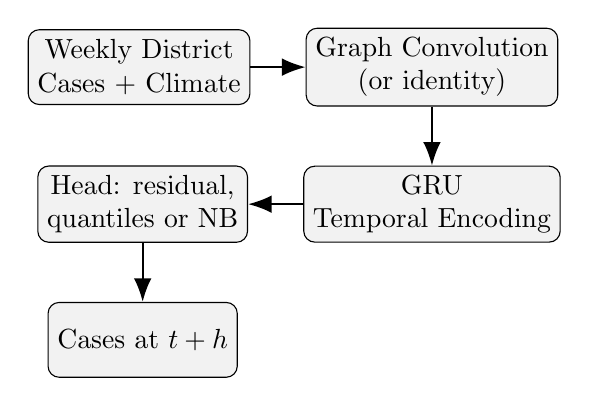
\begin{tikzpicture}[
    node distance=0.85cm,
    box/.style={draw, rounded corners, minimum width=2.0cm, minimum height=0.95cm, align=center, fill=gray!10},
    arrow/.style={-{Latex[length=3mm]}, thick}]
\node[box] (input) {Weekly District\\Cases + Climate};
\node[box, right=0.7cm of input] (gcn) {Graph Convolution\\(or identity)};
\node[box, below=0.75cm of gcn] (gru) {GRU\\Temporal Encoding};
\node[box, left=0.7cm of gru] (head) {Head: residual,\\quantiles or NB};
\node[box, below=0.75cm of head] (final) {Cases at $t+h$};
\draw[arrow] (input) -- (gcn);
\draw[arrow] (gcn) -- (gru);
\draw[arrow] (gru) -- (head);
\draw[arrow] (head) -- (final);
\end{tikzpicture}
\caption{The forecaster. The adjacency is identity (the GRU control), contiguity, Gaussian distance or learned; the head outputs one residual, seven quantiles or Negative Binomial parameters.}
\label{fig:pipeline}
\Description{Flow diagram: weekly district cases and climate pass through graph convolution or identity, then a GRU, then a head that outputs a residual, seven quantiles or Negative Binomial parameters, giving cases at week t plus h.}
\end{figure}

\subsection{Negative Binomial forecaster}
\label{sec:nb}
\textbf{Likelihood.} The head outputs a mean $\mu>0$ and dispersion $\alpha>0$ of an NB2 distribution, $\mathrm{E}[Y]=\mu$, $\mathrm{Var}[Y]=\mu+\alpha\mu^2$; training minimises the negative log-likelihood averaged over observed cells, and unobserved targets are masked.

\textbf{Mean link, zeros and initialisation.} The mean is anchored on the latest count, $\log\mu_{t,h}=\log(1+y_t)+\delta_{t,h}$, with $\delta$ clipped to $[-10,10]$. The $\delta$ projection is initialised at zero, so at initialisation $\mu=y_t+1$: one case above persistence, not persistence itself. Zero targets need no special treatment because the NB mass at zero, $(1+\alpha\mu)^{-1/\alpha}$, is positive; we make no zero-inflation assumption. The dispersion is $\alpha=\mathrm{softplus}(\cdot)+10^{-4}$, initialised near 0.69.

\textbf{Summaries.} The point forecast for MAE is the NB median, comparable to the median of the quantile models; the NB mean is reported separately. The same seven quantiles as every other probabilistic model are read from the NB distribution for WIS and coverage.

\textbf{Separate and shared variants.} The separate variant trains one model per horizon, exactly like the other GRU arms. The shared variant uses one GRU trunk with a parallel $(\mu,\alpha)$ head for each of the eight horizons, trained jointly. Each (origin, horizon) cell belongs to the split of its own target, so a training or validation origin never contributes a target from a later split; an earlier four-horizon implementation assigned origins by their one-week target and let validation origins carry test-year targets into early stopping, which this design removes.

\textbf{Ablations.} With v2 features and separate models, the squared-error, pinball and NB heads isolate the likelihood; with the NB head, separate and shared models isolate parameter sharing; with the shared NB model, v2, v3 and v4 isolate the inputs. Tuning effort and seeds are matched; parameter counts differ only by the heads (8{,}257 to 9{,}072; Table~\ref{tab:compute}).

\subsection{Baselines}
\textbf{Naive.} Persistence ($y_t$); seasonal naive ($y_{t+h-52}$); climatology (geometric mean of the same week in the previous five years); seasonal persistence (persistence shifted by the typical seasonal change from origin to target week).

\textbf{Tabular.} A global LightGBM~\cite{ke2017lightgbm} and a ridge autoregression (ARX) predict the same residual from v2 features, log-case lags 1--12, rolling means and maxima, lagged climate means, neighbour and national case levels, the target week's season and a district identifier.

\textbf{Foundation models.} Chronos-Bolt-small (checkpoint \texttt{amazon/chronos-bolt-small}) and Chronos-2 (\texttt{amazon/chronos-2})~\cite{ansari2024chronos,chronosbolt2024card,ansari2025chronos2} forecast $\log(1+y)$ from each district's full case history up to the origin (at most 1{,}011 weeks, within both models' context limits), with no task-specific parameter training (``zero-shot''). Chronos-2 is also run with past four-week climate means as past covariates and the target week's season as a known future covariate, and \emph{jointly}, with the 25 districts as one multivariate series. Fine-tuned variants apply LoRA per fold on data up to the training cut-off only, with a 512-week context; the number of steps (1{,}000 of $\{100,300,1000\}$) was chosen once on the 2015 validation year. We did not audit whether Chronos-2's pretraining corpus contains dengue series.

\textbf{Ensembles.} A pre-specified equal-weight ensemble of GRU~v2, LightGBM and Chronos-2 combined in log space; a stacked ensemble with non-negative least-squares weights and a top-3 ensemble chosen on the previous test year; and an equal-weight \emph{distribution} mixture of the shared NB model (its three seeds) and Chronos-2 joint, whose quantiles are solved from the mixed CDF, compared with averaging the two models' quantiles. The mixture's members were fixed before any result was seen.

\subsection{Evaluation protocol}
\textbf{Splits.} Walk-forward folds test each calendar year 2016--2026. For test year $Y$, validation targets are the periods starting in $Y-1$ (early stopping and variant selection) and training targets are all periods starting up to the end of $Y-2$. A cell is assigned to a split by its target week, so no training target crosses the training cut-off, although input windows may reach back into earlier splits. Imputation and scaling statistics use data before $Y$. Fold 0 (2016) is calibration only. The headline averages the seven non-COVID years 2017--2019 and 2022--2025; 2020--2021 are reported separately as a stress test. The 2026 fold (the first 19 weeks, 5 January--17 May) is a hold-out whose models, comparisons and success rule were declared on 29 September 2026 before any 2026 forecast was made (Section~\ref{sec:holdout}).

\textbf{Common cells.} Every method is scored on the same 223{,}000 (fold, split, horizon, week, district) cells, of which 108{,}200 are test cells. Anything calibrated for test year $f$ (conformal intervals, stacking weights, top-3 membership, alarm cutoffs) uses out-of-sample forecasts from year $f-1$ or earlier weeks already observed.

\textbf{Estimands and skill.} A trained model's score is the mean of its three per-seed scores; the score of the seed-averaged forecast is a different estimand, reported separately and never ranked against the first. Skill is the percentage reduction in headline mean MAE relative to same-horizon persistence, $1-\overline{\mathrm{MAE}}_{\text{model}}/\overline{\mathrm{MAE}}_{\text{persistence}}$, with means over the seven headline years; the mean of per-year percentage reductions can differ (for Chronos-2 joint at one week, 2.9\% against 6.3\%).

\textbf{Metrics.} MAE and peak MAE on raw counts, where peak cells are at or above the district's threshold, the 90th percentile of its pre-test history (a statistical, not an official, epidemic threshold); WIS~\cite{bracher2021evaluating}, 50/80/95\% coverage and interval width. Point models receive intervals from log-residuals in three ways: previous-year split conformal~\cite{vovk2005algorithmic}; rolling conformal, using the last 52 weeks of residuals already observed at the origin (a horizon-$h$ residual enters only after its target week is reported); and adaptive conformal~\cite{gibbs2021adaptive}, which updates each interval's miscoverage level weekly with step 0.05 fixed in advance.

\textbf{Statistics.} Paired $t$ and Wilcoxon tests over the seven headline years, per-year differences, and a time-block bootstrap (4-week blocks resampled jointly across all districts, 2{,}000 draws) that keeps the dependence between districts. With seven years the smallest attainable Wilcoxon $p$ is 0.016. Holm's procedure~\cite{holm1979simple} adjusts the declared primary family: the quantile level-weighted GRU, the shared NB model, Chronos-2 joint, LightGBM and the equal-weight ensemble against persistence at all eight horizons (40 tests). All other comparisons, including variant and feature searches, are exploratory. Because the 2017--2025 test years informed successive design choices, those results are retrospective and exploratory; the 2026 hold-out is the only untouched check.

%% ---------------------------------------------------------------------------
\section{One Week Ahead}
\label{sec:h1}

This section first summarises the earlier one-week experiments, which used the original polygon-mean climate extraction, and then the one-week results of the benchmark.

\begin{table}[t]
\centering
\caption{Earlier one-week study over the seven headline years (original climate extraction; not comparable cell-for-cell with Tables~\ref{tab:main}--\ref{tab:holdout}).}
\label{tab:h1baseline}
\begin{tabular}{lccccc}
\toprule
\textbf{Model} & \textbf{Feat.} & \textbf{MAE} & \textbf{RMSE} & \textbf{Peak} & \textbf{2017} \\
\midrule
Persistence & -- & \textbf{16.42} & \textbf{33.61} & \textbf{26.61} & \textbf{36.08} \\
GRU only & v1 & 16.68 & 35.25 & 28.06 & 42.97 \\
GRU only & v0 & 16.86 & 35.94 & 28.43 & 43.53 \\
GCN+GRU & v0 & 18.60 & 39.68 & 29.81 & 51.87 \\
GCN+GRU & v1 & 18.98 & 40.36 & 30.36 & 54.81 \\
\bottomrule
\end{tabular}
\end{table}

No trained model in the earlier study reduced headline mean MAE below persistence (Table~\ref{tab:h1baseline}). The GRU control beat the contiguity GCN--GRU on every fold. Figure~\ref{fig:h1} places every earlier configuration against persistence; each intervention changed mainly the 2017 epidemic year.
\begin{itemize}
\item \textbf{Learnable climate lags.} A per-district 26-week delay kernel recovered planted synthetic delays but not the observed 5--10-week lag association when trained end-to-end (learned vs observed $r=-0.16$; 20.67 MAE vs 18.36 for fixed windows). Sparse simplex activations in the kernel mixture (sparsemax, entmax) froze 58--74\% of kernels; a floored variant did not.
\item \textbf{Losses.} Level weighting cut GCN--GRU MAE from 18.98 to 16.59, entirely from 2017.
\item \textbf{Hyperparameters and optimisers.} A 50-trial search gained 0.75 MAE, under two seed standard deviations; AdamW~\cite{loshchilov2019decoupled} and plateau scheduling were within noise.
\item \textbf{Graphs.} No tested graph improved on the identity control (adaptive 16.61, identity 16.68, contiguity 18.98, Gaussian 19.25); a per-district gate between graph and identity learned almost nothing.
\end{itemize}

\begin{figure}[t]
\centering
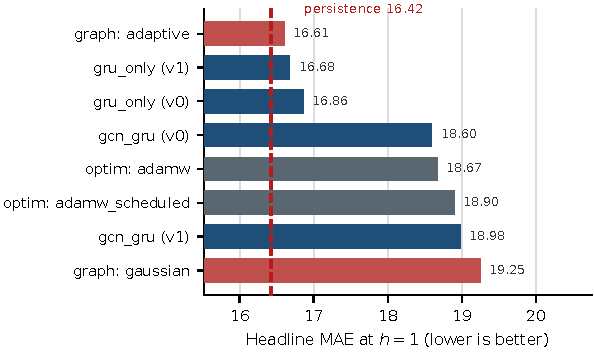
\includegraphics[width=\columnwidth]{fig_h1_landscape}
\caption{Every one-week configuration from the earlier study against persistence (dashed); original climate extraction.}
\label{fig:h1}
\Description{Horizontal bar chart of one-week MAE for every configuration from the earlier study; all bars sit at or to the right of the dashed persistence line at 16.42.}
\end{figure}

\textbf{One week in the benchmark.} Averaged over the six non-epidemic headline years, the learned models have lower one-week MAE than persistence (12.1--12.7 against 13.2); the headline mean is decided by 2017. A tested quantile-loss configuration, the quantile head with level weighting, reduced the headline mean error to 15.70 against 16.42 (six of seven years; paired $t$-test $p=0.045$, Wilcoxon $p=0.11$; block-bootstrap interval for the difference $[-1.14,-0.29]$); the evidence did not survive Holm correction over the primary family (adjusted $p=1.0$). The separate NB model reached 15.94 ($p=0.25$) and the shared NB model 16.63, above persistence; neither beat persistence in 2017 (37.52 and 40.30 against 36.08). The one-week result remains promising rather than established.

%% ---------------------------------------------------------------------------
\section{Multi-Horizon Benchmark}
\label{sec:benchmark}

Table~\ref{tab:main} gives headline MAE by horizon and Figure~\ref{fig:skill} the skill relative to same-horizon persistence, whose MAE rises from 16.42 at one week to 46.47 at twelve.

\begin{table*}[t]
\centering
\caption{Headline MAE (cases per district-week; mean over the seven headline test years of the mean of three seeds) by horizon $h$ in weeks. Bold marks the lowest value per column. All rows are scored on identical cells.}
\label{tab:main}
\begin{tabular}{llcccccccc}
\toprule
\textbf{Family} & \textbf{Method} & $h=1$ & $h=2$ & $h=3$ & $h=4$ & $h=6$ & $h=8$ & $h=10$ & $h=12$ \\
\midrule
Naive & Persistence & 16.42 & 20.16 & 24.58 & 28.47 & 35.01 & 40.07 & 43.76 & 46.47 \\
 & Seasonal persistence & 23.19 & 26.36 & 30.16 & 32.90 & 37.20 & 42.66 & 45.04 & 48.16 \\
Tabular & Ridge ARX & 17.96 & 21.39 & 24.24 & 26.70 & 30.96 & 34.22 & 36.52 & 38.23 \\
 & LightGBM & 16.99 & 21.05 & 24.30 & 27.16 & 32.34 & 36.29 & 38.14 & 40.59 \\
GRU & GRU v2, squared error & 16.64 & 19.51 & 22.33 & 25.30 & 30.85 & 34.33 & 36.96 & 38.10 \\
 & GRU v2, pinball & 15.93 & 19.23 & 22.43 & 25.06 & 29.48 & 33.28 & 35.92 & 37.77 \\
 & GRU v2, pinball + level-weighted & \textbf{15.70} & 19.00 & 22.38 & 24.58 & 29.94 & 33.10 & 35.83 & 37.94 \\
 & GRU v2, NB (separate) & 15.94 & 19.26 & 22.46 & 25.07 & 29.83 & 31.94 & 36.75 & 40.25 \\
 & GRU v2, NB (shared trunk) & 16.63 & 19.83 & 23.15 & 25.84 & 30.25 & 33.46 & 35.86 & 37.67 \\
 & GCN v2 (contiguity graph) & 17.84 & 23.30 & 25.46 & 27.59 & 31.86 & 34.58 & 37.36 & 38.78 \\
Foundation & Chronos-Bolt, zero-shot & 16.60 & 20.19 & 23.63 & 26.41 & 30.50 & 33.42 & 35.36 & 36.69 \\
 & Chronos-2, zero-shot & 16.03 & 19.34 & 22.85 & 25.89 & 30.46 & 33.98 & 36.37 & 37.63 \\
 & Chronos-2 joint, zero-shot & 15.95 & 19.07 & 22.29 & 25.11 & 29.39 & 32.74 & 34.91 & 36.29 \\
 & Chronos-2 joint, fine-tuned & 17.32 & 19.80 & 22.38 & 25.07 & 28.82 & 31.70 & 33.86 & 35.17 \\
 & Chronos-2, fine-tuned & 18.59 & 21.07 & 23.59 & 25.63 & 29.26 & 31.74 & \textbf{33.58} & \textbf{34.76} \\
Ensemble & Equal weights (pre-specified) & 16.05 & 19.27 & 22.30 & 25.01 & 29.79 & 33.19 & 35.35 & 36.81 \\
 & Top-3 by previous year & 15.92 & 19.87 & 23.14 & 25.15 & 29.62 & 32.58 & 36.01 & 36.48 \\
 & Mixture NB + Chronos-2 joint & 15.78 & \textbf{18.79} & \textbf{21.85} & \textbf{24.49} & \textbf{28.59} & \textbf{31.69} & 33.88 & 35.30 \\
\bottomrule
\end{tabular}
\end{table*}

\begin{figure*}[t]
\centering
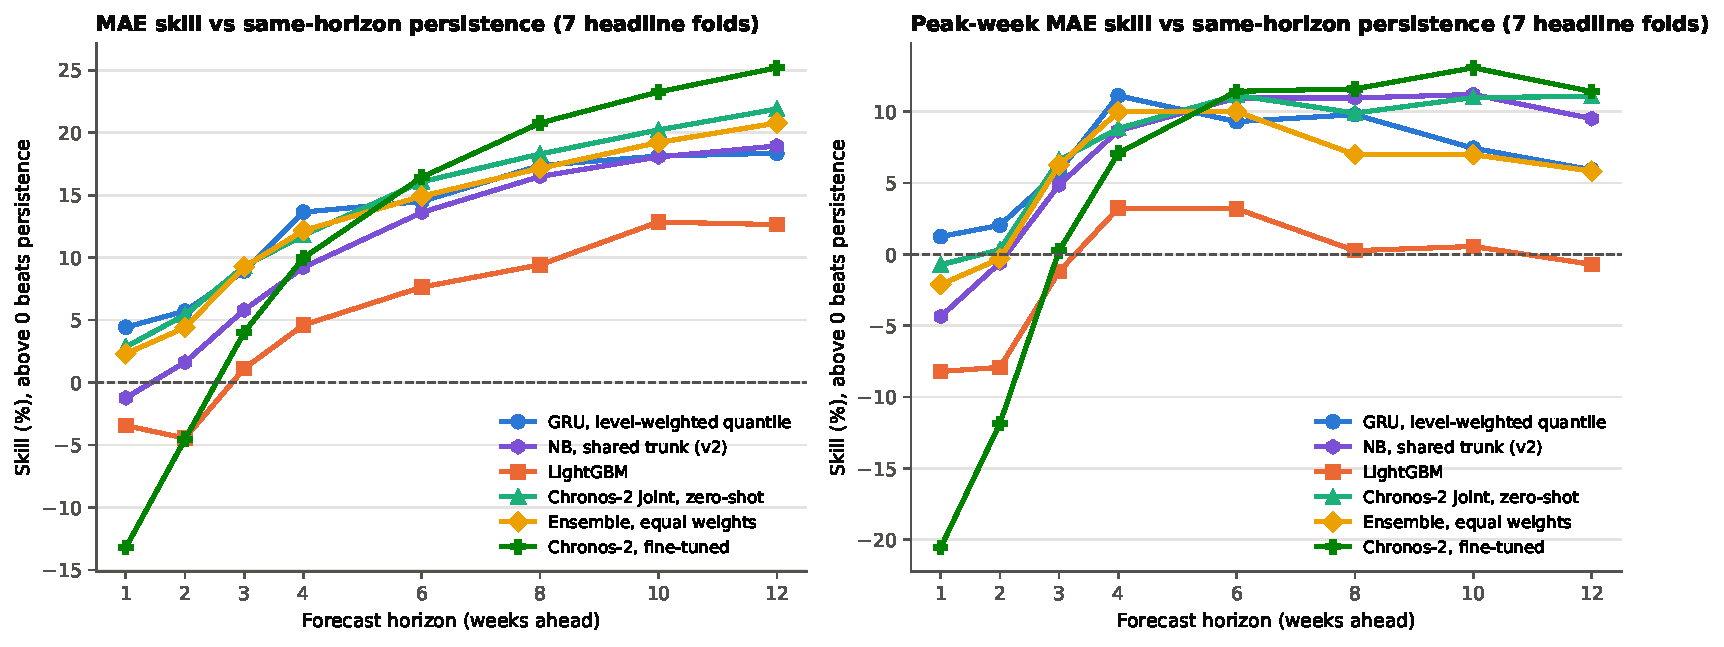
\includegraphics[width=\textwidth]{fig_lh_skill}
\caption{Skill relative to same-horizon persistence for MAE (left) and peak-week MAE (right), headline years. Above zero beats persistence.}
\label{fig:skill}
\Description{Two line charts of skill versus forecast horizon from 1 to 12 weeks for six forecasters. Most lines start near zero at one week and rise to between 12 and 25 percent at 12 weeks.}
\end{figure*}

\textbf{Skill grows with horizon.} From three weeks most learned models have lower MAE than persistence, and the margin grows: at four weeks the quantile level-weighted GRU has 13.6\% skill and the equal-weight ensemble 12.2\%; at twelve weeks skill is 18--25\% (fine-tuned Chronos-2 25.2\%, the mixture 24.0\%, Chronos-2 joint 21.9\%, the shared NB model 18.9\%). The block bootstrap excludes zero for the quantile level-weighted GRU, Chronos-2 joint and the ensemble from four weeks on, and Chronos-2 joint and the ensemble win all seven years from three weeks (Wilcoxon $p=0.016$). After Holm correction over the 40 primary tests only Chronos-2 joint at three weeks remains significant (adjusted $p=0.025$): seven years give low power, and the horizon-level evidence rests on consistency across years, horizons and model families rather than on individual tests.

\textbf{Foundation models.} Chronos-2 evaluated without task-specific fine-tuning, using only the context available at each origin, was within about 0.6 MAE of the best GRU at every horizon; joint forecasting of the 25 districts improved on univariate Chronos-2 at every horizon by 0.1--1.5 MAE. Fine-tuning moves skill toward long horizons but costs 2.6 MAE at one week, almost all in 2017, which the model, fine-tuned on quieter years, under-predicts.

\textbf{Tabular baselines and ensembles.} LightGBM does not beat persistence at one or two weeks and trails the GRU by 2--3 MAE from four weeks; the linear ARX is competitive at long horizons. Stacked weights are worse than equal weights at every horizon, and the top-3 membership changes between years, an instance of the forecast-combination puzzle. The NB--Chronos-2 mixture has the lowest MAE from two to eight weeks and beats the NB model in all seven years at every horizon.

\textbf{COVID years.} In 2020--2021, when transmission and reporting were disrupted, the learned models again beat persistence at every reported horizon (at four weeks 10.8--12.2 MAE against 14.2; at twelve weeks 15.6--23.0 against 30.0), with LightGBM and the NB model among the strongest.

%% ---------------------------------------------------------------------------
\section{The Negative Binomial Model}
\label{sec:nbresults}

\begin{table}[t]
\centering
\caption{Controlled NB ablations: MAE change (row minus reference; negative favours the row), headline years. Footnote: point forecasts are NB medians unless stated.}
\label{tab:nb}
\small
\setlength{\tabcolsep}{3pt}
\begin{tabular}{lcccc}
\toprule
\textbf{Comparison} & $h$=1 & 4 & 8 & 12 \\
\midrule
\multicolumn{5}{l}{\emph{Likelihood (v2, separate models)}} \\
Pinball vs squared error & $-0.71$ & $-0.24$ & $-1.05$ & $-0.34$ \\
NB vs squared error & $-0.70$ & $-0.23$ & $-2.39$ & $+2.15$ \\
NB vs pinball & $+0.01$ & $+0.01$ & $-1.34$ & $+2.49$ \\
\multicolumn{5}{l}{\emph{Sharing (NB, v2)}} \\
Shared trunk vs separate & $+0.69$ & $+0.77$ & $+1.52$ & $-2.59$ \\
\multicolumn{5}{l}{\emph{Features (shared NB)}} \\
v3 vs v2 & $+0.54$ & $+0.80$ & $+0.45$ & $-0.13$ \\
v4 vs v2 & $+0.64$ & $+1.09$ & $+0.89$ & $+0.40$ \\
v4, centre chosen on validation vs 28\,$^\circ$C & $-0.15$ & $-0.29$ & $-0.45$ & $-0.54$ \\
\multicolumn{5}{l}{\emph{Point summary (shared NB)}} \\
Mean vs median & $-0.02$ & $+0.68$ & $+1.37$ & $+1.87$ \\
\bottomrule
\end{tabular}
\end{table}

\textbf{Likelihood.} With features, backbone and budget fixed, the NB head matched the pinball head within 0.04 MAE up to four weeks (Table~\ref{tab:nb}); neither differed significantly from the other at any horizon. The NB head was better at eight weeks and worse at twelve, where the separate NB model's error grew. A count likelihood is therefore a sound alternative to quantile regression on this task but did not improve on it.

\textbf{Sharing and features.} One shared trunk for all horizons was 0.6--0.8 MAE worse than separate models up to four weeks and better only at ten and twelve, while needing one eighth of the training fits (Table~\ref{tab:compute}). Neighbour-case features (v3) and hand-lagged biological features (v4) did not improve the shared NB model at any horizon up to ten weeks. Choosing the thermal centre per fold on the validation year (it selected 26--30\,$^\circ$C, most often 26\,$^\circ$C) recovered 0.15--0.54 MAE of v4's deficit, but v4 remained worse than v2.

\textbf{Point summary and calibration.} The NB median beats the NB mean from four weeks, increasingly with horizon, because the mean of a right-skewed distribution overshoots typical weeks. The NB model's predicted share of zero counts is close to the observed share (0.042--0.048 predicted against 0.038 observed at one week), so a zero-inflated model is not needed. Its 80\% intervals cover 0.89 of cells at one week and 0.81 at twelve, but coverage falls on peak weeks (95\% intervals: 0.94 at one week, 0.72--0.76 at twelve) and in 2017 (0.66--0.74 at twelve weeks); district-level 80\% coverage ranges from 0.70 to 0.90 at twelve weeks. Average coverage near nominal therefore hides under-coverage in epidemic weeks. Unlike an earlier four-horizon report, the NB model on these common cells did not beat persistence in all seven years at one week.

%% ---------------------------------------------------------------------------
\section{What Climate Contributes}
\label{sec:climate}

\textbf{Design.} Three controls are used and described separately. A \emph{climatology} control replaces every climate channel by each district's week-of-year mean over the training years only, keeping width and architecture; comparing full weather with it asks whether observed weather adds information beyond a seasonal calendar of weather. A \emph{removal} control drops the channels. A \emph{shuffle} control permutes each climate channel in time, independently per district and channel, keeping width and marginal distributions; because it also breaks the relations between weather variables and their rolling means, its penalty is a secondary diagnostic, not a clean causal estimate. Chronos-2 is compared with and without climate covariates. We apply the climatology and removal controls to the GRU, the shared NB model and LightGBM.

\begin{table}[t]
\centering
\caption{Incremental predictive value of observed weather: MAE of the control minus MAE with observed weather (positive means observed weather helps), headline years.}
\label{tab:climate}
\small
\setlength{\tabcolsep}{3pt}
\begin{tabular}{llccccc}
\toprule
\textbf{Model} & \textbf{Control} & $h$=1 & 2 & 4 & 8 & 12 \\
\midrule
GRU & climatology & $+0.44$ & $+1.03$ & $+1.32$ & $+1.42$ & $+1.48$ \\
 & removed & $+0.03$ & $+1.32$ & $+2.22$ & $+1.94$ & $+2.49$ \\
NB shared & climatology & $+0.30$ & $+0.58$ & $+0.99$ & $+1.35$ & $+1.26$ \\
 & removed & $+1.45$ & $+1.76$ & $+2.31$ & $+3.01$ & $+3.26$ \\
LightGBM & climatology & $+0.07$ & $+0.34$ & $+0.18$ & $+0.46$ & $+0.25$ \\
 & removed & $+0.40$ & $+0.64$ & $+0.63$ & $+0.47$ & $+0.52$ \\
Chronos-2 & covariates & $-0.68$ & $-0.22$ & $+0.96$ & $+1.60$ & $+1.78$ \\
NB shared & weather 1 week late & $+0.01$ & $-0.17$ & $-0.27$ & $-0.03$ & $+0.21$ \\
\bottomrule
\end{tabular}
\end{table}

\begin{figure*}[t]
\centering
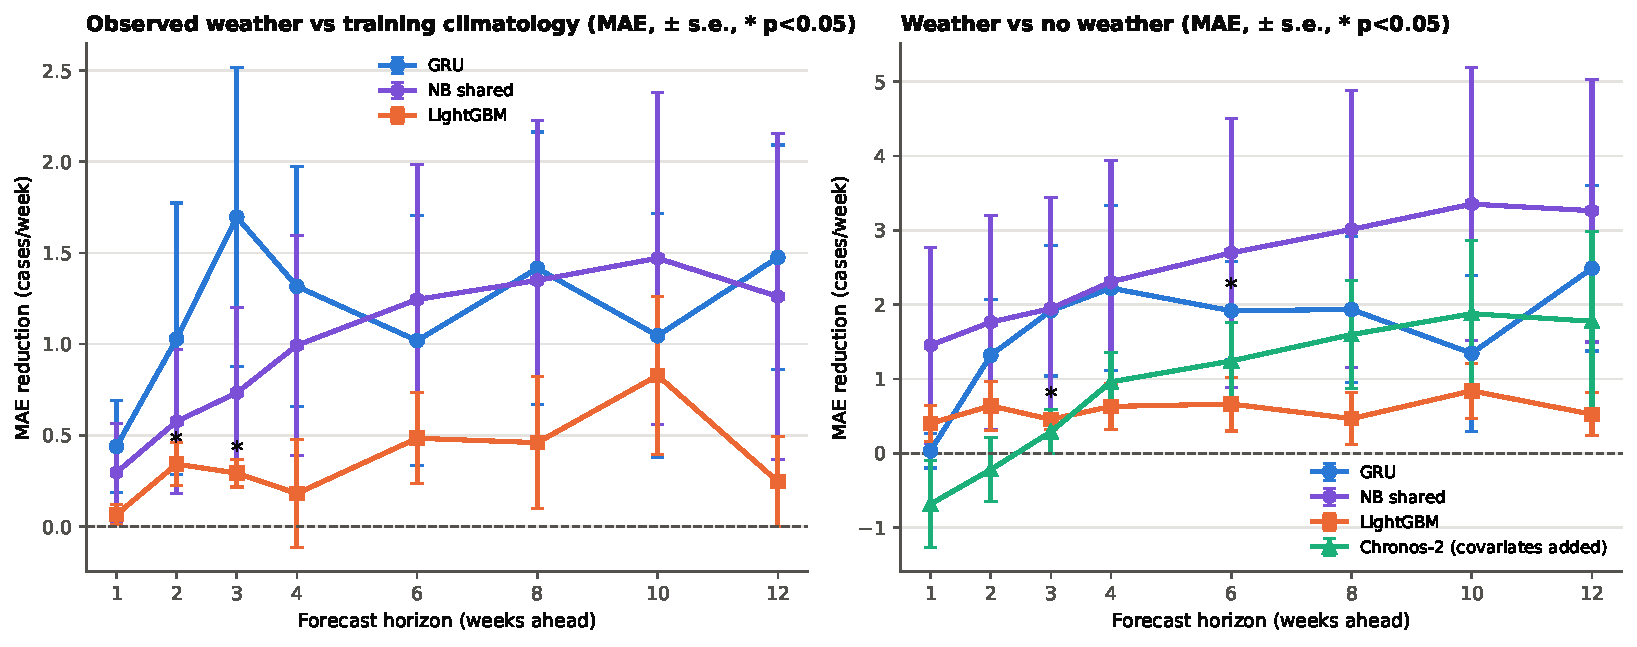
\includegraphics[width=\textwidth]{fig_lh_climate}
\caption{Incremental predictive value of weather by horizon: observed weather against a training-years climatology (left) and against no weather (right), MAE, $\pm$ standard error over seven headline years; * paired $p<0.05$.}
\label{fig:climate}
\Description{Two line charts versus horizon. Left: reduction in MAE from observed weather over a climatology of weather for a GRU, an NB model and LightGBM, positive at every horizon. Right: reduction from any weather over none, including Chronos-2 with covariates, negative at one and two weeks for Chronos-2 and positive elsewhere.}
\end{figure*}

\textbf{Results.} Observed past weather improved accuracy beyond the training-period climatology in all three families at every horizon (Table~\ref{tab:climate}, Figure~\ref{fig:climate}): by 0.4--1.7 MAE for the GRU, 0.3--1.5 for the NB model and 0.1--0.8 for LightGBM. Full weather beat the climatology in four to six of seven years for the GRU at every horizon, and the block bootstrap excludes zero at all horizons for the GRU and NB models; individual paired tests over years are mostly at $p=0.05$--0.3. From two weeks, removing climate costs more than replacing it with climatology, so part of what climate channels carry is seasonal phase and part is the weather actually observed. Delaying weather by one week changed MAE by at most 0.27, so the result does not depend on the most recent week of weather. Chronos-2 is hurt by climate covariates at one and two weeks and helped from four.

\textbf{Interpretation.} These are measures of incremental predictive value, not causal effects. The effect does not fade by twelve weeks, beyond the observed 5--10-week lag association; weather at the origin may also encode the phase and strength of the monsoon season. A compact distributed-lag basis~\cite{gasparrini2010dlnm,lowe2018barbados} fitted on validation data is a natural next comparison with the fixed rolling windows used here.

%% ---------------------------------------------------------------------------
\section{Spatial Structure}
\label{sec:spatial}

\begin{table}[t]
\centering
\caption{MAE change from adding a graph to the GRU~v2 control (positive means the graph variant is worse).}
\label{tab:graphs}
\begin{tabular}{lccccc}
\toprule
\textbf{Graph} & $h=1$ & $h=2$ & $h=4$ & $h=8$ & $h=12$ \\
\midrule
Contiguity & $+1.20$ & $+3.78$ & $+2.29$ & $+0.25$ & $+0.68$ \\
Learned (adaptive) & $+0.49$ & $+5.58$ & $+1.61$ & $+1.61$ & $+1.27$ \\
\bottomrule
\end{tabular}
\end{table}

The tested contiguity and learned graph variants did not improve headline MAE over the matched GRU control under this protocol at any horizon (Table~\ref{tab:graphs}); the learned graph's learning rate was selected per fold and horizon on the validation year. The contiguity penalty shrinks with horizon but does not become a gain. Neighbour-case features given to the NB model (v3) did not help either (Section~\ref{sec:nbresults}), so neither graph mixing nor these simple spatial predictors improved on the temporal model; ``no graph convolution'' is not ``no spatial information'', since v3 and v4 carry neighbour cases. Joint Chronos-2 forecasting improved on univariate Chronos-2; because the two differ in model family, this does not isolate an effect of attention over message passing. With 25 nodes and strongly district-specific dynamics, the tested graphs may add smoothing where little is warranted; this is a hypothesis, not an established cause.

%% ---------------------------------------------------------------------------
\section{Probabilistic Forecasts}
\label{sec:probabilistic}

\begin{table}[t]
\centering
\caption{WIS (lower is better), 95\% coverage and mean 95\% width (cases), headline years; 2017 is the 95\% coverage in the epidemic year at $h=12$. ``prev.'' = previous-year conformal, ``roll.'' = rolling conformal, ``adapt.'' = adaptive conformal.}
\label{tab:wis}
\small
\setlength{\tabcolsep}{2.5pt}
\begin{tabular}{lccccccc}
\toprule
& \multicolumn{3}{c}{\textbf{WIS}} & \multicolumn{2}{c}{\textbf{Cov.\ 95\%}} & \textbf{Width} & \textbf{2017} \\
\textbf{Method} & $h$=1 & 4 & 12 & 4 & 12 & 12 & 12 \\
\midrule
Persistence, prev. & 12.51 & 19.66 & 33.46 & 0.96 & 0.95 & 640 & 0.95 \\
Persistence, adapt. & 11.54 & 27.33 & 47.91 & 0.95 & 0.95 & 1549 & 0.95 \\
LightGBM, prev. & 10.47 & 18.39 & 39.57 & 0.93 & 0.85 & 404 & 0.62 \\
LightGBM, roll. & 10.29 & 17.23 & 35.56 & 0.95 & 0.90 & 436 & 0.75 \\
LightGBM, adapt. & 10.23 & 18.87 & 59.93 & 0.95 & 0.95 & 1143 & 0.90 \\
GRU pinball + LW & 9.18 & \textbf{14.38} & 25.40 & 0.95 & 0.91 & 189 & 0.67 \\
NB shared & 9.97 & 15.78 & 23.79 & 0.94 & 0.92 & 157 & 0.75 \\
Chronos-2 joint & \textbf{9.08} & 14.74 & 22.74 & 0.95 & 0.93 & 182 & 0.82 \\
Chronos-2 joint, FT & 9.95 & 14.89 & \textbf{22.28} & 0.96 & 0.95 & 206 & 0.82 \\
Mixture NB + Chronos-2 & 9.29 & 14.73 & 22.40 & 0.93 & 0.91 & 189 & 0.81 \\
\bottomrule
\end{tabular}
\end{table}

\begin{figure*}[t]
\centering
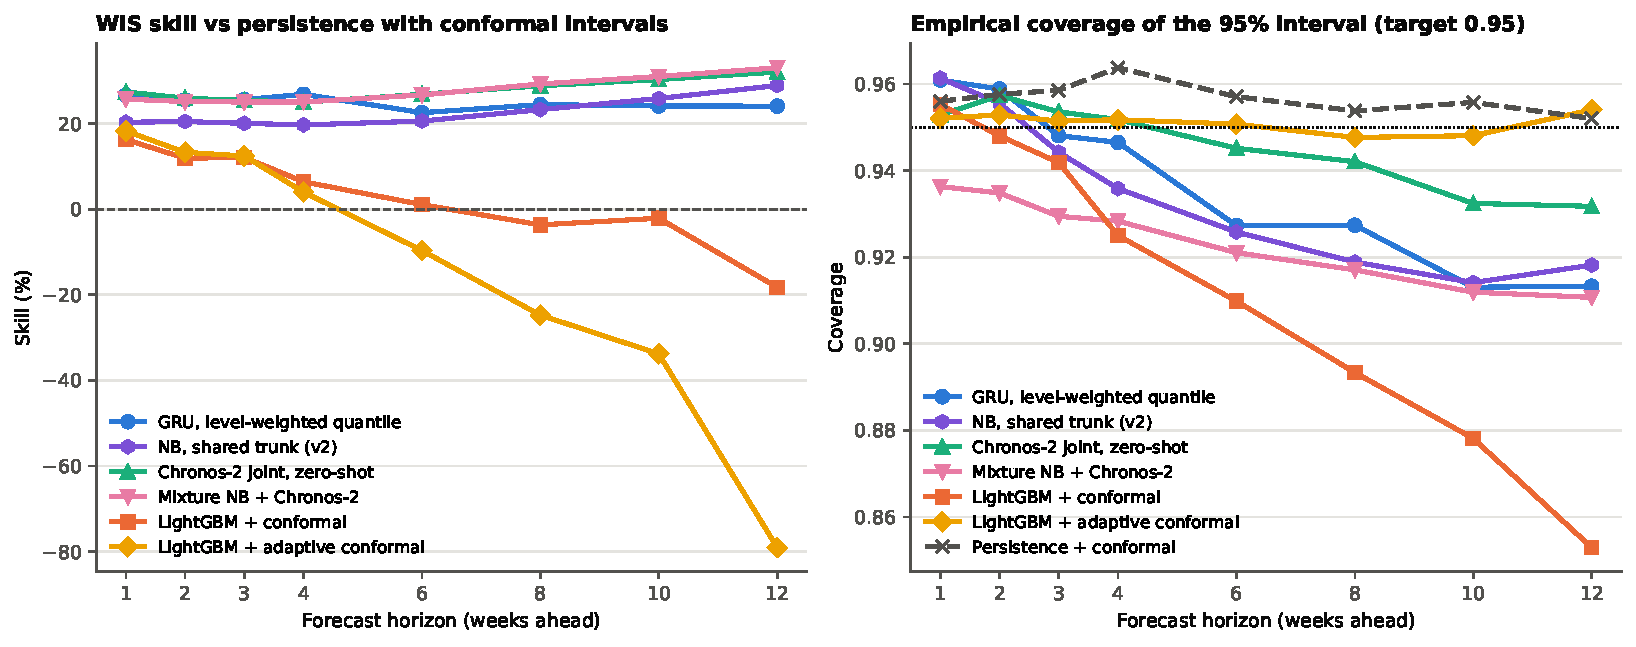
\includegraphics[width=\textwidth]{fig_lh_probabilistic}
\caption{WIS skill relative to persistence with previous-year conformal intervals (left) and 95\% coverage (right, target dotted), headline years.}
\label{fig:probabilistic}
\Description{Left: WIS skill versus horizon; native quantile and NB forecasts sit near 20 to 33 percent, LightGBM with conformal intervals falls below zero at long horizons, and adaptive conformal falls further. Right: coverage versus horizon, with previous-year conformal intervals for LightGBM falling to 0.85 at 12 weeks and adaptive conformal holding near 0.95.}
\end{figure*}

\begin{figure*}[t]
\centering
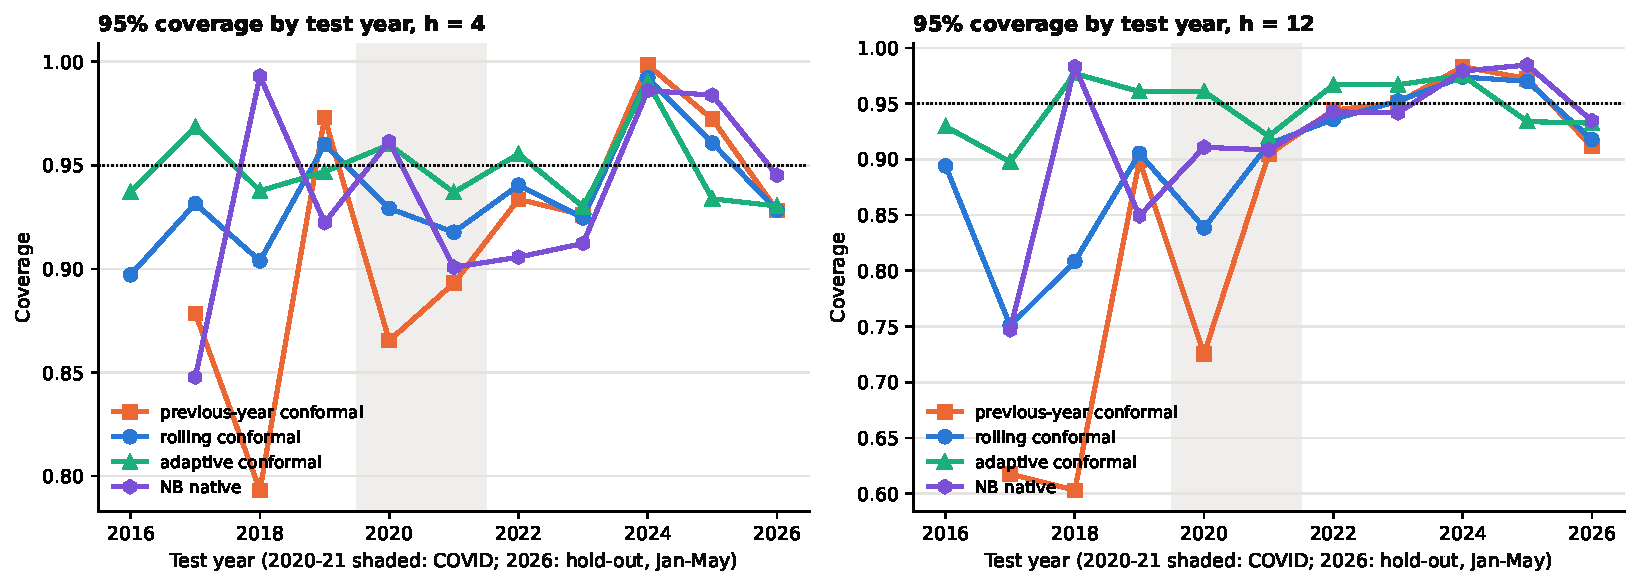
\includegraphics[width=\textwidth]{fig_lh_coverage_by_year}
\caption{95\% coverage by test year at four and twelve weeks for LightGBM with three conformal calibrations and for the native NB model; 2020--21 shaded; 2026 is the January--May hold-out.}
\label{fig:coverage}
\Description{Two line charts of coverage by year from 2016 to 2026. Previous-year conformal coverage drops to about 0.6 in 2017 and 2018 at twelve weeks; adaptive conformal stays between 0.9 and 0.98 in every year; rolling conformal and the NB model fall to about 0.75 in 2017.}
\end{figure*}

\textbf{Native forecasts.} Native quantile and NB forecasts improve WIS over persistence by 20--27\% at one and four weeks and by 24--33\% at twelve (Table~\ref{tab:wis}), with average 95\% coverage of 0.91--0.96. The NB model has the narrowest intervals at long horizons. The NB--Chronos-2 mixture is close to the best single model at every horizon; averaging the two models' quantiles gives almost the same WIS (22.41 at twelve weeks) and point accuracy, so here the mixture's distributional form mattered little.

\textbf{Calibration under change.} Average coverage conceals the epidemic year: at twelve weeks every native interval, and the previous-year conformal intervals of the trained models, under-cover 2017 (0.62--0.82 against 0.95; Figure~\ref{fig:coverage}). Rolling conformal, which uses the latest residuals already observed, improves LightGBM's WIS at every horizon (35.56 against 39.57 at twelve weeks) and its coverage. Adaptive conformal holds 0.95 coverage at every horizon and 0.87--0.99 in every year, including 2017, but its intervals become several times wider at long horizons and its WIS is worse: nominal coverage in every regime is bought with sharpness. The choice between them depends on whether guaranteed coverage or informative width matters more to the user.

%% ---------------------------------------------------------------------------
\section{Early Warning: Outbreak Weeks and Onsets}
\label{sec:ews}

\textbf{Two event definitions.} An \emph{outbreak week} is a district-week at or above the district's threshold; outbreak-week discrimination scores every forecaster on all test weeks. \emph{Onset prediction} is a separate task with its own population. An origin is \emph{at risk} if the district's last four weeks, the origin included, are observed and below threshold; the label is whether the first threshold crossing occurs within the next $K$ weeks ($K=4$ or 8). Every comparator is scored on the same eligible origins, whose $K$ target weeks all lie in the test year: 5{,}265 origins at $K=4$ (20.6\% positive) and 4{,}872 at $K=8$ (33.3\% positive) over the headline years, containing 215 onset events. A point forecaster's window score is its largest forecast-to-threshold ratio over the horizons inside the window; a probabilistic forecaster's score is its largest marginal exceedance probability, a lower bound on the window probability, never a product of marginals. A LightGBM classifier is trained on the onset label, with and without climate, and a seasonal base rate from pre-test years is a reference. Alarm cutoffs are set on the previous test year so that 10\% of eligible origins alarm. Each onset is counted once: it is detected if any eligible origin in the $K$ weeks before it alarmed, with lead time from the earliest alarm.

\begin{table}[t]
\centering
\caption{Onset prediction at $K=4$ weeks over the headline years (5{,}265 at-risk origins, 20.6\% positive, 215 onsets). Brier is shown for probabilities; for forecasters it is the Brier score of the largest marginal exceedance probability (a lower bound). FA = false alarms per district-year at the previous-year cutoff.}
\label{tab:ews}
\small
\setlength{\tabcolsep}{3pt}
\begin{tabular}{lccccc}
\toprule
\textbf{Method} & \textbf{ROC} & \textbf{PR} & \textbf{Brier} & \textbf{Detected} & \textbf{FA} \\
\midrule
Persistence & 0.70 & 0.36 & -- & 0.57 & 3.8 \\
Seasonal base rate & 0.66 & 0.34 & 0.169 & 0.27 & 2.0 \\
Onset classifier & 0.76 & 0.45 & \textbf{0.134} & 0.50 & 5.0 \\
Onset classifier, no climate & 0.74 & 0.41 & 0.143 & 0.48 & 4.8 \\
LightGBM & 0.74 & 0.41 & -- & \textbf{0.61} & 4.4 \\
GRU pinball + LW & 0.76 & 0.44 & 0.138 & 0.58 & 3.5 \\
NB shared & 0.75 & 0.44 & 0.142 & 0.54 & 4.1 \\
Chronos-2 joint & 0.75 & 0.45 & 0.142 & 0.48 & 3.8 \\
Chronos-2 joint, FT & \textbf{0.77} & \textbf{0.47} & 0.138 & 0.51 & 3.5 \\
\bottomrule
\end{tabular}
\end{table}

\begin{figure*}[t]
\centering
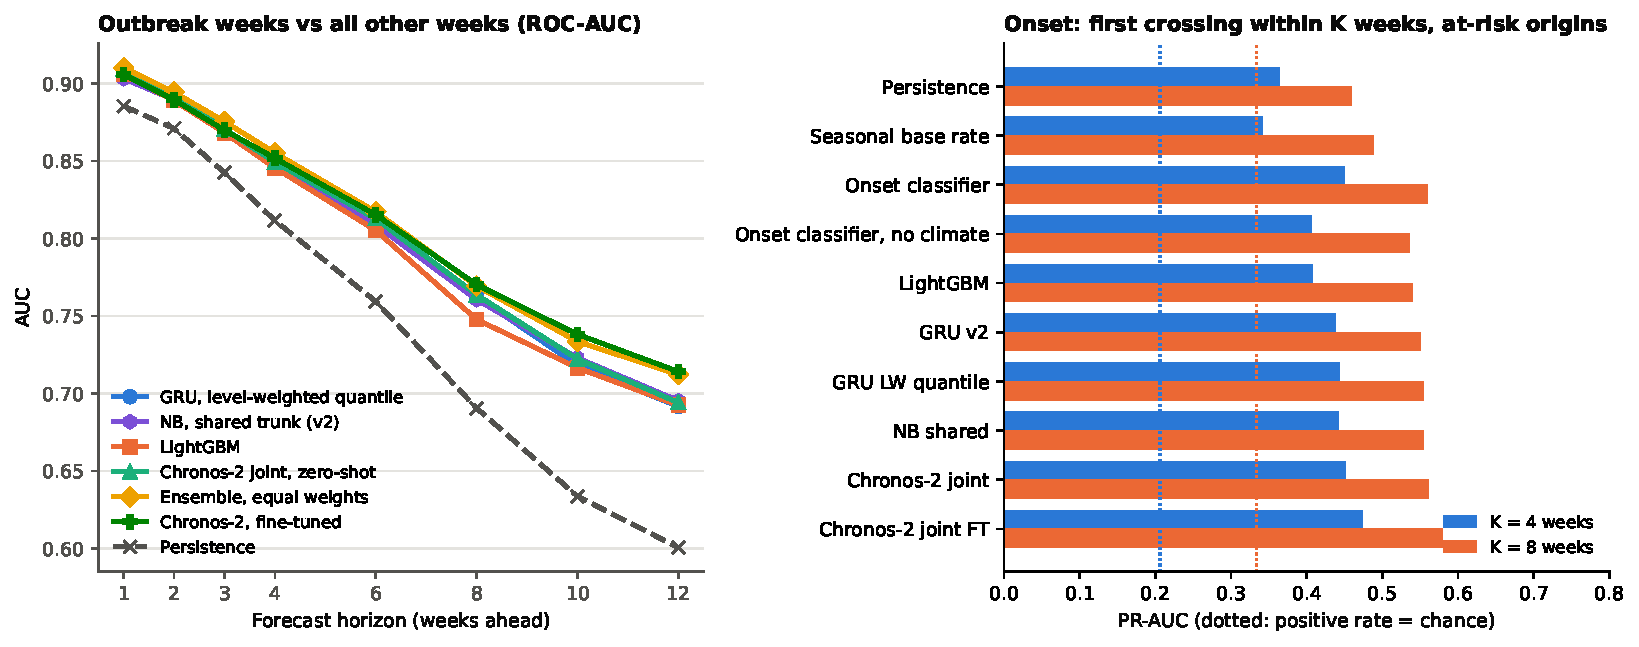
\includegraphics[width=\textwidth]{fig_lh_early_warning}
\caption{Left: ROC-AUC for outbreak weeks against all other weeks by horizon. Right: onset prediction on at-risk origins, PR-AUC at $K=4$ and 8 weeks; dotted lines mark the positive rate (chance).}
\label{fig:ews}
\Description{Left: outbreak-week ROC-AUC falling from about 0.91 at one week to about 0.7 at twelve for learned models and from 0.89 to 0.60 for persistence. Right: horizontal bars of onset PR-AUC for ten methods, between 0.34 and 0.47 at four weeks and 0.46 to 0.58 at eight weeks, all above the positive-rate lines of 0.21 and 0.33.}
\end{figure*}

\textbf{Outbreak weeks.} Learned models discriminate outbreak weeks at ROC-AUC 0.90--0.91 one week ahead against 0.89 for persistence, and the gap widens with horizon (0.68--0.71 against 0.60 at twelve weeks; Figure~\ref{fig:ews}). High scores here largely reflect outbreaks already under way.

\textbf{Onsets.} On the at-risk population the tested models showed moderate onset discrimination with the available predictors and this event definition (Table~\ref{tab:ews}): ROC-AUC 0.74--0.77 and PR-AUC 0.41--0.47 at four weeks against a 0.21 positive rate, above persistence (0.70, 0.36) and the seasonal base rate (0.66, 0.34). The onset classifier gave the best-calibrated probabilities (Brier 0.134 against 0.169 for the base rate), and climate improved it (PR-AUC 0.45 against 0.41). At the previous-year cutoff the models detected 48--61\% of onsets with a median lead of three weeks at $K=4$ (four to six at $K=8$), at a cost of 3.5--5.0 false alarms per district-year. The realised alarm rate was 0.18 against the 0.10 budget, again reflecting year-to-year non-stationarity. An earlier evaluation that scored onset weeks against all quiet weeks, with a different population from its classifier, reported onset AUC of 0.53--0.63; that comparison mixed two tasks and is superseded here. A model comparison of this kind does not establish a limit on onset predictability.

%% ---------------------------------------------------------------------------
\section{Hold-out Year and Computational Cost}
\label{sec:holdout}

\begin{table}[t]
\centering
\caption{2026 hold-out (19 weeks, January--May), declared before forecasting: MAE and the difference from persistence with a 95\% time-block bootstrap interval.}
\label{tab:holdout}
\small
\setlength{\tabcolsep}{2.5pt}
\begin{tabular}{lccc}
\toprule
\textbf{Method} & $h$=1 & $h$=4 & $h$=12 \\
\midrule
Persistence & 17.60 & 22.47 & 30.68 \\
GRU pinball + LW & 15.46 {\scriptsize$[-3.9,-0.6]$} & 19.94 {\scriptsize$[-5.3,0.0]$} & 23.62 {\scriptsize$[-15.2,0.5]$} \\
NB shared & 16.26 {\scriptsize$[-4.1,1.1]$} & 20.68 {\scriptsize$[-6.0,1.9]$} & 27.40 {\scriptsize$[-10.8,4.7]$} \\
Chronos-2 joint & 14.34 {\scriptsize$[-7.7,-0.04]$} & 19.18 {\scriptsize$[-8.3,1.8]$} & 27.03 {\scriptsize$[-10.2,2.9]$} \\
LightGBM & 15.77 {\scriptsize$[-5.2,0.9]$} & 21.39 {\scriptsize$[-4.4,2.3]$} & 28.98 {\scriptsize$[-8.1,5.4]$} \\
Equal-weight ensemble & 14.96 {\scriptsize$[-5.5,-0.2]$} & 19.53 {\scriptsize$[-6.0,-0.2]$} & 26.19 {\scriptsize$[-10.1,1.7]$} \\
\bottomrule
\end{tabular}
\end{table}

\textbf{Hold-out.} All five declared models had lower MAE than persistence at all eight horizons in 2026 (Table~\ref{tab:holdout}), consistent in sign with the 2017--2025 results. With 19 weeks most bootstrap intervals include zero; they exclude it at one week for the quantile level-weighted GRU, Chronos-2 joint and the ensemble, at four weeks for the ensemble, and at six weeks for the GRU and the ensemble. The window covers the first transmission peak of the year but not the monsoon peak.

\begin{table}[t]
\centering
\caption{Computational cost on one laptop (NVIDIA RTX 4070 Laptop, 8\,GB; LightGBM on CPU). Fits cover 11 folds $\times$ 8 horizons $\times$ 3 seeds unless shared; inference per forecast origin (25 districts).}
\label{tab:compute}
\small
\setlength{\tabcolsep}{2.5pt}
\begin{tabular}{lrrrr}
\toprule
\textbf{Model} & \textbf{Params} & \textbf{s/fit} & \textbf{ms/origin} & \textbf{GPU MB} \\
\midrule
GRU v2, squared error & 8{,}257 & 1.2 & 0.02 & 141 \\
GRU v2, pinball + LW & 8{,}455 & 1.9 & 0.02 & 141 \\
GRU v2, NB (separate, 264 fits) & 8{,}290 & 2.2 & 0.02 & 141 \\
NB shared (33 fits) & 8{,}752 & 2.4 & 0.02 & 143 \\
LightGBM (CPU) & -- & 0.7 & -- & -- \\
Chronos-Bolt-small & 47.7M & -- & 38.5 & 2{,}162 \\
Chronos-2, zero-shot & 119.5M & -- & 30.5 & 1{,}123 \\
Chronos-2 joint, LoRA & 120.7M & 180 & 33.8 & 2{,}911 \\
\bottomrule
\end{tabular}
\end{table}

\textbf{Computation.} The GRU and NB forecasters have 8--9 thousand parameters, train in 1--2.5 seconds per fit and forecast in about 0.02\,ms per origin; Chronos-2 has 119.5 million parameters and needs about 30\,ms per origin and 1--3\,GB of GPU memory (Table~\ref{tab:compute}). The tuning budget was a 50-trial search for the GRU (inherited, not repeated), none for the NB heads, early stopping for LightGBM, five ridge penalties and three fine-tuning lengths for Chronos-2, each selected on validation data only.

%% ---------------------------------------------------------------------------
\section{Discussion}

\textbf{Case forecasting and outbreak warning.} The current results support different conclusions for case forecasting and outbreak warning. Longer-horizon forecasts improve on persistence, but these improvements do not by themselves establish reliable detection of new outbreaks; on a consistent at-risk definition, onset discrimination was moderate and came with several false alarms per district-year. The tested graph variants also did not improve on the matched temporal control. These findings concern the evaluated models and data; they do not imply that spatial transmission is absent or that onset prediction cannot improve with other predictors or modelling choices.

\textbf{Agreement with prior work.} The graph result agrees with Gogovi~\cite{gogovi2026spatial} and contrasts with GNN gains reported against weaker baselines and without an identity-graph control~\cite{weng2024graph,gulmohamed2026denguegnn}. The climate result agrees with the delayed associations reported for Sri Lanka and Barbados~\cite{liu2025explainable,lowe2018barbados}, while showing that part of what climate channels carry is seasonal phase. That forecasts beat persistence mainly beyond two weeks is consistent with operational experience that skill is horizon-specific~\cite{colongonzalez2021probabilistic}.

\textbf{What the small model contributes.} A compact persistence-anchored GRU matched or approached a 119-million-parameter pretrained model at every horizon while training in seconds on a laptop, and its likelihood mattered less than its horizon and its inputs: the pinball and NB heads were interchangeable, while observed weather helped consistently. Combining the NB model with Chronos-2 gave the best point accuracy from two to eight weeks. Fine-tuning the foundation model on pre-epidemic years lowered its robustness to the 2017 regime change.

\textbf{Limitations.} The benchmark climate is a centroid-based reconstruction retrieved in 2026, not the values available at each origin, and case-reporting delays are not modelled. The 2017--2025 test years informed successive design choices, so those results are exploratory and retrospective; seven headline years give low power, and after Holm correction only one primary comparison is individually significant. The hold-out covers 19 weeks. Chronos fine-tuning was tuned on one validation year, and the pretraining corpus was not audited for dengue series. The outbreak threshold is statistical, not official.

%% ---------------------------------------------------------------------------
\section{Conclusion}

For 25 Sri Lankan districts, the tested learned forecasters improved on persistence mainly from three to twelve weeks ahead, reaching 18--25\% lower MAE at twelve weeks and 24--33\% lower WIS, a pattern that the declared 2026 hold-out reproduced in sign. A compact persistence-anchored GRU with a quantile or Negative Binomial head performed comparably to a pretrained foundation model at a small fraction of its cost; the Negative Binomial head matched but did not improve on quantile regression. Observed weather improved accuracy beyond a climatology of weather, and the tested graph variants did not help. Onset prediction was moderately discriminative on a consistent definition but produced frequent false alarms. These conclusions are limited to the tested models, data and horizons. Future work should validate the frozen specification prospectively with the NDCU, model input availability and reporting delays, compare distributed-lag climate bases, and test onset-specific data such as mobility, entomological and serotype surveillance. Retrospective AUC alone does not establish operational readiness.

\bibliographystyle{ACM-Reference-Format}
\bibliography{references_long}

\end{document}
